\documentclass{standalone}

\usepackage{tikz}

\begin{document}
  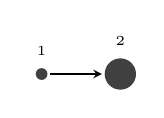
\begin{tikzpicture}
    \tikzstyle{v1} = [color=darkgray, circle, outer sep=1pt, fill, inner sep=1.5pt]
    \tikzstyle{v3} = [color=darkgray, circle, outer sep=1pt, fill, inner sep=4.0pt]
    \tikzstyle{e} = [->, >={stealth}] \tikzset{font=\tiny}

    \node[v1, label={1}] (1) at (0,0) {};
    \node[v3, label={2}] (2) at (1,0) {};
    \draw[e] (1) -- (2);
  \end{tikzpicture}
\end{document}
